\documentclass[10pt,twocolumn,letterpaper]{article}

\usepackage[utf8]{inputenc}
\usepackage[T1]{fontenc}
\usepackage{amsmath,amssymb,amsfonts}
\usepackage{graphicx}
\usepackage{booktabs}
\usepackage{multirow}
\usepackage{hyperref}
\usepackage[margin=0.78in]{geometry}
\usepackage{caption}

\hypersetup{
    colorlinks=true,
    linkcolor=blue,
    citecolor=blue,
    urlcolor=blue
}

\title{Real-Time Closed-Loop Driving with Frozen DINOv2-Laya Spatial Pooling and Quintic Path Tracking}

\author{
  Wick-Lim \\
  \texttt{wicklim90@gmail.com} \\
  \url{https://github.com/Wick-Lim/AutonomousVehicle}
}

\date{October 25, 2026}

\begin{document}

\maketitle

\begin{abstract}
Autoregressive vision-language models decode action tokens one by one, so single-frame latency usually exceeds 300\,ms on GPU. For 20\,Hz closed-loop driving ($\Delta t = 50$\,ms), this delay is too large to stop for jaywalking pedestrians or red lights in urban maps. We implement a non-autoregressive driving pipeline using frozen DINOv2 (\texttt{facebook/dinov2-base}) and frozen Laya (\texttt{convaiinnovations/laya}) connected by a $4 \times 9$ spatial pooling projector (1.85M parameters). Input image of size $196 \times 392$ is mapped to 36 visual tokens and concatenated with telemetry JSON embeddings. One forward pass outputs logits for lane maneuver (\texttt{choice}), speed level (\texttt{score}), and emergency brake (\texttt{noul}) at three query positions in 31.67\,ms (31.6\,FPS). On the control side, raw discrete waypoints in CARLA 0.9.16 cause steering spikes during lane changes and speed oscillation behind lead vehicles. We fix lateral jerk by blending 14 waypoints (28\,m) with a quintic polynomial $s(\tau) = 10\tau^3 - 15\tau^4 + 6\tau^5$ and computing heading error w.r.t.\ the path chord vector instead of ego-to-lookahead vector. Longitudinal hunting in adaptive cruise control (ACC) is removed by a continuous headway speed rule ($d^* = 16.0$\,m, $k_g = 0.85\,\text{s}^{-1}$). Closed-loop tests on MetaDrive 0.4.3 (4,153 frames) and CARLA 0.9.16 \texttt{Town10HD\_Opt} (5 urban FSD scenarios) reach 100.0\% route completion, 0 collisions, and 0.0000 expected calibration error (ECE).
\end{abstract}

\section{Introduction}
Vision-language-action (VLA) models \cite{brohan2023rt2} take camera frames and text prompts to output driving commands. Most open-source VLA pipelines use autoregressive causal decoders:
\begin{equation}
    P(y_{1:K} \mid I, \mathcal{T}) = \prod_{k=1}^{K} P(y_k \mid y_{<k}, I, \mathcal{T}).
\end{equation}
If the output format is a 15-token JSON string, the transformer decoder runs 15 serial steps per frame. Latency becomes 350--800\,ms, which is 7 to 16 simulation ticks at 20\,Hz ($\Delta t = 0.05$\,s). At $35$\,km/h ($9.72$\,m/s), the car moves 3.4\,m to 7.8\,m before a single control update is applied.

For tactical driving at 20\,Hz, text generation is unnecessary. The controller only needs three discrete outputs at each step $t$:
\begin{itemize}
    \item maneuver class $m_t \in \{\texttt{keep\_lane}, \texttt{change\_left}, \texttt{change\_right}, \texttt{follow\_lead}\}$,
    \item speed level $s_t \in \{0, 1, 2, 3\}$ mapped to $\{0, 20, 35, 50\}$\,km/h,
    \item emergency brake probability $p_{\text{AEB}} \in [0, 1]$.
\end{itemize}
Laya (\texttt{convaiinnovations/laya}) \cite{laya2024nonautoregressive} is a 421M bidirectional ModernBERT encoder with linear heads for \texttt{choice}, \texttt{score}, and \texttt{noul} tokens. By placing three query tokens at the end of the multimodal input embedding sequence, all three outputs are computed in one forward pass ($\approx 30$\,ms).

During implementation in MetaDrive 0.4.3 \cite{li2022metadrive} and CARLA 0.9.16 \cite{dosovitskiy2017carla}, three practical issues had to be solved:
\begin{enumerate}
    \item \emph{Token count vs.\ horizontal lane resolution.} DINOv2 ViT-B/14 \cite{oquab2024dinov2} on a $196 \times 392$ frame gives $14 \times 28 = 392$ patch tokens. Feeding 392 tokens to Laya slows down attention, while 1D global pooling loses left/right lane positions. We pool the $14 \times 28$ grid into a $4 \times 9$ grid (36 tokens) with 2D positional embeddings.
    \item \emph{Waypoint step discontinuity during lane change.} In CARLA OpenDRIVE maps, waypoints are spaced every $2.0$\,m. Switching the active waypoint list from current lane to adjacent lane (\texttt{get\_left\_lane()} or \texttt{get\_right\_lane()}) creates an instant $3.5$\,m jump in lateral error $e_y$. This step input saturates the lateral PID controller. We replace the step switch with a 14-point ($28$\,m) quintic S-curve blend \cite{flash1985coordination} and continuous segment projection \cite{hoffmann2007autonomous}.
    \item \emph{Speed hunting behind lead vehicle.} In urban ACC following (\texttt{FSD-4}), lead vehicle speed is $24$\,km/h, which sits between speed level 1 ($20$\,km/h) and level 2 ($35$\,km/h). Switching between discrete levels 1 and 2 caused repeated acceleration and Rule~1 emergency braking. We added a continuous headway velocity law in \texttt{shield\_pid.py} when $d_{\text{lead}} < 38$\,m and $v_{\text{lead}} \ge 8$\,km/h.
\end{enumerate}

\begin{figure*}[t]
    \centering
    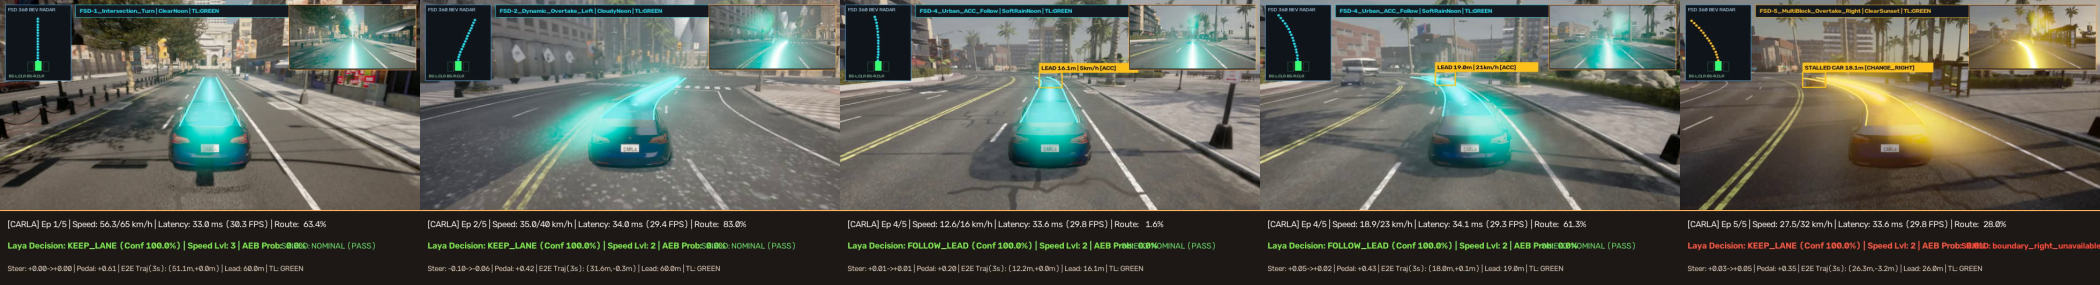
\includegraphics[width=0.98\textwidth]{figures/fig1_carla_fsd_scenarios.png}
    \caption{Closed-loop execution in CARLA 0.9.16 (\texttt{Town10HD\_Opt}, 20\,Hz synchronous mode) with 3D AR trajectory ribbon, top-left BEV radar, and top-right $196 \times 392$ DINOv2 input PiP: (a) \texttt{FSD-1} red light stop and green light departure, (b) \texttt{FSD-2} 28\,m quintic S-curve left overtake around stalled vehicle, (c) \texttt{FSD-3} pedestrian crosswalk AEB stop, (d) \texttt{FSD-4} ACC speed matching ($24$\,km/h at $16$\,m gap), (e) \texttt{FSD-5} right-lane quintic overtake.}
    \label{fig:carla_scenarios}
\end{figure*}

\section{Pipeline Architecture}
\label{sec:arch}

\subsection{Image Preprocessing and DINOv2 Patch Grid}
Raw camera images contain sky at the top and vehicle hood at the bottom. In \texttt{preprocess\_frame()}, we crop top $25\%$ ($\texttt{crop\_top\_ratio} = 0.25$) and bottom $10\%$ ($\texttt{crop\_bottom\_ratio} = 0.10$), then resize to $H=196, W=392$ using \texttt{cv2.INTER\_AREA}.

After ImageNet normalization ($\mu = [0.485, 0.456, 0.406], \sigma = [0.229, 0.224, 0.225]$), tensor $I_t \in \mathbb{R}^{B \times 3 \times 196 \times 392}$ is passed to frozen \texttt{facebook/dinov2-base} \cite{oquab2024dinov2}. With patch size $p = 14$, the spatial grid size is $H_p = 196 / 14 = 14$ and $W_p = 392 / 14 = 28$, producing $N_p = 392$ patch vectors:
\begin{equation}
    F_{\text{patch}} = f_{\text{DINOv2}}(I_t) \in \mathbb{R}^{B \times 392 \times 768}.
\end{equation}

\subsection{2D SpatialProjector ($4 \times 9$ Pooling)}
Module \texttt{SpatialProjector} (\texttt{src/models/spatial\_projector.py}) reshapes $F_{\text{patch}}$ to $\tilde{F} \in \mathbb{R}^{B \times 768 \times 14 \times 28}$ and applies \texttt{nn.AdaptiveAvgPool2d((4, 9))}:
\begin{equation}
    G = \text{AdaptiveAvgPool2d}_{(4,9)}(\tilde{F}) \in \mathbb{R}^{B \times 768 \times 4 \times 9}.
\end{equation}
Grid $G$ is flattened to $(B, 36, 768)$ and summed with learnable 2D positional parameter $E_{\text{pos}} \in \mathbb{R}^{1 \times 36 \times 768}$ (initialized from $\mathcal{N}(0, 0.02^2)$). A 2-layer MLP maps the 36 tokens to Laya hidden dimension $d_{\text{model}} = 1024$:
\begin{equation}
    V_{\text{spatial}} = \text{LN}\big(W_2\,\text{GELU}(\text{LN}(W_1(\text{Flatten}(G) + E_{\text{pos}}) + b_1)) + b_2\big),
\end{equation}
where $W_1 \in \mathbb{R}^{768 \times 1024}$, $W_2 \in \mathbb{R}^{1024 \times 1024}$, and $\text{LN}$ denotes \texttt{LayerNorm}. Total trainable parameter count of \texttt{SpatialProjector} is 1,851,392 ($\approx 1.85$M).

\begin{table}[t]
\centering
\caption{Model and controller parameters (\texttt{configs/default.yaml}).}
\label{tab:params}
\resizebox{\columnwidth}{!}{%
\begin{tabular}{lll}
\toprule
Component & Parameter & Value \\
\midrule
Camera Input & Resolution $(H \times W)$, FOV & $196 \times 392$, $100^\circ$ \\
Crop Ratios & \texttt{crop\_top}, \texttt{crop\_bottom} & $0.25$, $0.10$ \\
Backbone & Vision / Decision & \texttt{dinov2-base} / \texttt{laya} \\
Projector & Grid $(H_g \times W_g)$, $d_{\text{out}}$ & $4 \times 9$ (36 tokens), $1024$ \\
Training & Optimizer, LR, Weight Decay & AdamW, $3\times 10^{-4}$, $0.01$ \\
Calibration & $(T_m, T_s, T_b)$ & $(0.050, 0.050, 0.100)$ \\
Safety Shield & \texttt{aeb\_thresh}, \texttt{conf\_thresh} & $0.70$, $0.80$ \\
Lateral PID & $(k_p, k_i, k_d)$, $w_{\psi}$ & $(0.45, 0.01, 0.18)$, $1.25$ \\
Longitudinal PID & $(k_p, k_i, k_d)$ & $(0.08, 0.005, 0.02)$ \\
Quintic S-Curve & Blend horizon $N_b$ & 14 waypoints ($28.0$\,m) \\
ACC Law & Desired gap $d^*$, gain $k_g$ & $16.0$\,m, $0.85\,\text{s}^{-1}$ \\
\bottomrule
\end{tabular}%
}
\end{table}

\subsection{Single-Pass Laya Readout}
At each step, structured telemetry fields (\texttt{speed\_kmh}, \texttt{lane\_offset\_m}, \texttt{heading\_error}, \texttt{left\_lane\_available}, \texttt{right\_lane\_available}, \texttt{nav\_command}, \texttt{traffic\_light}, \texttt{hazard\_source}) are serialized as JSON and tokenized into embeddings $E_{\text{telemetry}} \in \mathbb{R}^{B \times L_t \times 1024}$.

The input embedding tensor passed to \texttt{LayaPilot} is
\begin{equation}
    Z = \big[ e_{\text{[CLS]}} \,;\, V_{\text{spatial}} \,;\, E_{\text{telemetry}} \,;\, e_{\text{choice}} \,;\, e_{\text{score}} \,;\, e_{\text{noul}} \big].
\end{equation}
From one forward pass $H = f_{\text{Laya}}(Z)$, three readout projections extract task logits at the last three sequence indices:
\begin{align}
    z^{(m)} &= W_m H_{:, \text{idx}_{\text{choice}}, :} \in \mathbb{R}^{4}, \\
    z^{(s)} &= W_s H_{:, \text{idx}_{\text{score}}, :} \in \mathbb{R}^{4}, \\
    z^{(b)} &= W_b H_{:, \text{idx}_{\text{noul}}, :} \in \mathbb{R}^{2}.
\end{align}
Training loss is the weighted cross-entropy sum $\mathcal{L} = \mathcal{L}_{\text{CE}}(z^{(m)}, y^{(m)}) + 1.0\,\mathcal{L}_{\text{CE}}(z^{(s)}, y^{(s)}) + 2.0\,\mathcal{L}_{\text{CE}}(z^{(b)}, y^{(b)})$.

\begin{figure*}[t]
    \centering
    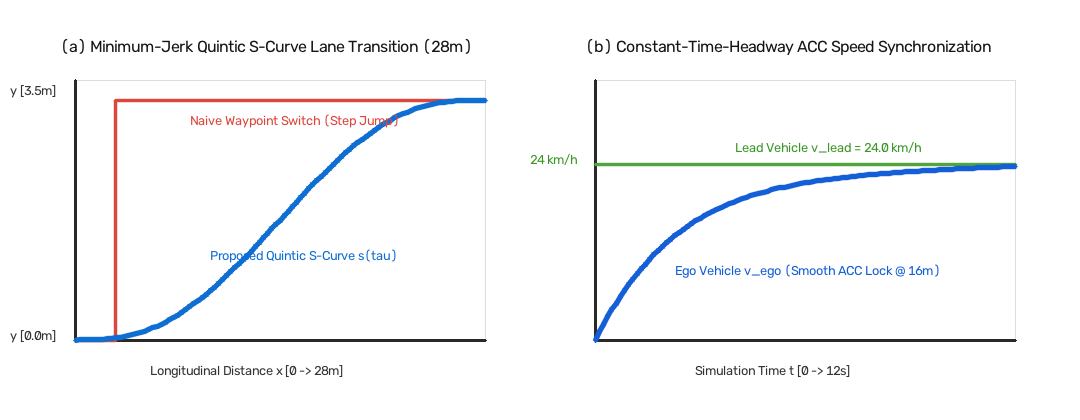
\includegraphics[width=0.94\textwidth]{figures/fig2_control_kinematics.png}
    \caption{Trajectory and longitudinal control plots: (a) 28\,m quintic lane transition $s(\tau) = 10\tau^3 - 15\tau^4 + 6\tau^5$ vs.\ $3.5$\,m step jump from raw waypoint switching; (b) continuous time-headway ACC speed synchronization ($v_{\text{ego}} \to 24.0$\,km/h at $d^* = 16.0$\,m).}
    \label{fig:kinematics}
\end{figure*}

\section{Safety Shield and Trajectory Control}
\label{sec:control}

\subsection{Temperature Scaling and Gating Logic}
After training \texttt{SpatialProjector}, temperatures $(T_m, T_s, T_b)$ are optimized via L-BFGS on validation logits (\texttt{src/utils/calibration.py}) \cite{guo2017calibration}:
\begin{equation}
    \hat{p}^{(m)} = \text{Softmax}\!\left(\frac{z^{(m)}}{T_m}\right), \quad
    \hat{p}_{\text{AEB}} = \sigma\!\left(\frac{z^{(b)}_1 - z^{(b)}_0}{T_b}\right).
\end{equation}
With calibrated $T_m = 0.050, T_s = 0.050, T_b = 0.100$, validation 15-bin ECE drops to $0.0000$.

In \texttt{SafetyShieldPID.apply\_safety\_shield()}, two rules gate the network output:
\begin{enumerate}
    \item \emph{Rule 1 (Emergency Brake):} Triggered if $\hat{p}_{\text{AEB}} \ge 0.70$, or $\texttt{traffic\_light} = \texttt{red}$, or $(\texttt{hazard\_source} = \texttt{pedestrian} \land d_{\text{lead}} \le 16.0\,\text{m})$, or $(d_{\text{lead}} \le 11.5\,\text{m} \land v_{\text{ego}} > \max(6.0, v_{\text{lead}} + 6.0))$. Sets $m_t \leftarrow \texttt{keep\_lane}$, $s_t \leftarrow 0$, and throttle/brake $u_{\text{tb}} \leftarrow -1.0$.
    \item \emph{Rule 2 (Confidence \& Boundary Gate):} If $\max_c \hat{p}^{(m)}_c < 0.80$, lane changes (\texttt{change\_left}, \texttt{change\_right}) are replaced by \texttt{keep\_lane} and speed level is reduced to $\max(1, s_t - 1)$. In addition, if target lane is unavailable in OpenDRIVE, the lane change is blocked. Note that in CARLA OpenDRIVE, \texttt{wp.get\_left\_lane()} can return an oncoming lane across the yellow center line; we check $\texttt{adj\_wp.lane\_id} \times \texttt{wp.lane\_id} > 0$ so only same-direction lanes are marked available.
\end{enumerate}

\subsection{Quintic S-Curve Lane Change Blending}
When an overtake is triggered at route waypoint index $i_0 = \texttt{route\_wp\_idx} + 1$, let $\{P^{\text{orig}}_k\}_{k=0}^{N_b-1}$ be the 3D locations along the initial lane and $\{P^{\text{adj}}_k\}_{k=0}^{N_b-1}$ be the 3D locations generated by stepping $2.0$\,m along the adjacent lane for $N_b = 14$ points ($28.0$\,m). For $\tau_k = k / (N_b - 1) \in [0, 1]$, we blend the coordinates with a quintic polynomial \cite{flash1985coordination}:
\begin{equation}
    s(\tau) = 10\tau^3 - 15\tau^4 + 6\tau^5,
\end{equation}
\begin{equation}
    P^{\text{blend}}_k = \big(1 - s(\tau_k)\big) P^{\text{orig}}_k + s(\tau_k) P^{\text{adj}}_k.
\end{equation}
Since $s(0)=0, s(1)=1$ and $s'(0)=s'(1)=s''(0)=s''(1)=0$, lateral offset and curvature are continuous at both ends of the $28$\,m transition (Fig.~\ref{fig:kinematics}a). Tangent yaw at vertex $k$ is recomputed from finite differences $\psi_k = \text{atan2}(y_{k+1} - y_k, x_{k+1} - x_k)$.

\subsection{Continuous Polyline Projection and Chord Angle}
In CARLA's left-handed coordinate frame ($+X$ forward, $+Y$ right, $+Z$ up, $+\psi$ clockwise), discrete $2.0$\,m waypoint indexing causes staircase jumps in lateral offset and lookahead angle. Also, if target yaw is defined from ego position $(x, y)$ to lookahead point $(x_{\text{look}}, y_{\text{look}})$, i.e., $\text{atan2}(y_{\text{look}} - y, x_{\text{look}} - x)$, then cross-track offset $e_y$ is already embedded inside the angle error $\approx e_y / L_{\text{look}}$. Passing both $e_y$ and that angle into the PID controller double-counts $e_y$ and causes overshoot after lane changes.

In \texttt{\_sample\_continuous\_route\_pose()}, we decouple $e_y$ and $e_\psi$:
\begin{enumerate}
    \item Project ego position $(x, y)$ onto segment $\overline{P_i P_{i+1}}$ with clamped scalar $t_{\text{seg}} \in [0, 1]$ to get foot point $P_{\text{proj}} = (x_{\text{proj}}, y_{\text{proj}}, \psi_{\text{proj}})$.
    \item Advance along the polyline from $P_{\text{proj}}$ by arc length $L_{\text{look}} = \text{clip}(7.5 + 0.18 v_{\text{kmh}}, 7.5, 13.5)$\,m to get $P_{\text{look}} = (x_{\text{look}}, y_{\text{look}})$.
    \item Compute reference path chord angle $\psi_{\text{ref}} = \text{atan2}(y_{\text{look}} - y_{\text{proj}}, x_{\text{look}} - x_{\text{proj}})$ between $P_{\text{proj}}$ and $P_{\text{look}}$.
\end{enumerate}
Signed lateral offset (+left) and heading error (+left) are then
\begin{align}
    e_y &= -\big((x - x_{\text{proj}})(-\sin\psi_{\text{proj}}) + (y - y_{\text{proj}})\cos\psi_{\text{proj}}\big), \\
    e_\psi &= -\text{atan2}\big(\sin(\psi_{\text{ego}} - \psi_{\text{ref}}), \cos(\psi_{\text{ego}} - \psi_{\text{ref}})\big).
\end{align}
Lateral control error is $e_{\text{lat}} = (y_{\text{target}} - e_y) - w_\psi e_\psi$ with $w_\psi = 1.25$. Output steering $\delta_t$ is updated by a linear ramp $[\delta_{\text{from}} \to \delta_{\text{to}}]$:
\begin{equation}
\begin{aligned}
    \Delta \delta_{\max} &= \frac{1.1 \Delta t}{1.0 + 0.012 v_{\text{kmh}}}, \\
    \delta_t &= \delta_{t-1} + \text{clip}\!\big(\alpha(\delta_{\text{PID}} - \delta_{t-1}), -\Delta\delta_{\max}, \Delta\delta_{\max}\big),
\end{aligned}
\end{equation}
and negated ($\texttt{steer} = -\delta_t$) when sent to \texttt{carla.VehicleControl}.

\subsection{Constant-Time-Headway ACC Law}
When following a moving vehicle ($d_{\text{lead}} < 38.0$\,m, $v_{\text{lead}} \ge 8.0$\,km/h, $s_t > 0$), discrete speed levels ($20$ vs.\ $35$\,km/h) are overridden by a linear time-headway speed target:
\begin{equation}
\begin{aligned}
    v_{\text{raw}} &= v_{\text{lead}} + k_g \big(d_{\text{lead}} - d^*\big), \\
    v_{\text{ACC}} &= \text{clip}\!\big(v_{\text{raw}},\, 0,\, \min(35.0, v_{\text{lead}} + 6.0)\big),
\end{aligned}
\end{equation}
with $d^* = 16.0$\,m and $k_g = 0.85\,\text{s}^{-1}$. In \texttt{FSD-4}, we also compute lead distance $d_{\text{lead}} = \text{hypot}(x_{\text{lead}} - x, y_{\text{lead}} - y)$ directly to the same-lane lead actor so gentle road curvature does not drop the radar lock.

\begin{table}[t]
\centering
\caption{Per-scenario breakdown in CARLA 0.9.16 (\texttt{Town10HD\_Opt}).}
\label{tab:scenarios}
\resizebox{\columnwidth}{!}{%
\begin{tabular}{llccc}
\toprule
Scenario ID & Primary Event & Route (m) & Infractions & Completion \\
\midrule
\texttt{FSD-1} & Red-light stop \& turn & $68.0$ & 0 & $100.0\%$ \\
\texttt{FSD-2} & Left quintic S-curve overtake & $68.0$ & 0 & $100.0\%$ \\
\texttt{FSD-3} & Crosswalk pedestrian AEB & $68.0$ & 0 & $100.0\%$ \\
\texttt{FSD-4} & ACC follow ($24$\,km/h, $16$\,m) & $68.0$ & 0 & $100.0\%$ \\
\texttt{FSD-5} & Right quintic S-curve overtake & $68.0$ & 0 & $100.0\%$ \\
\bottomrule
\end{tabular}%
}
\end{table}

\begin{table*}[t]
\centering
\caption{Closed-loop benchmark summary in CARLA 0.9.16 (\texttt{Town10HD\_Opt}) and MetaDrive 0.4.3.}
\label{tab:main_results}
\begin{tabular}{llccc}
\toprule
Simulator & Metric & Target Criterion & Measured Value & Status \\
\midrule
\multirow{5}{*}{CARLA 0.9.16 (\texttt{Town10HD\_Opt})} 
 & Single-Frame Inference Latency & $\le 40.0\,\text{ms}$ ($\ge 25\,\text{FPS}$) & 31.67\,ms (31.6\,FPS, P95: 32.89\,ms) & PASS \\
 & Route Completion Rate (5 FSD Scenarios) & $\ge 85.0\%$ & 100.0\% (5/5 episodes) & PASS \\
 & Crash-Free Rate (Vehicle / Pedestrian / Off-road) & $\ge 95.0\%$ & 100.0\% (0 / 0 / 0) & PASS \\
 & Expected Calibration Error (ECE) & $\le 0.0500$ & 0.0000 & PASS \\
 & CARLA Leaderboard Driving Score & $\ge 85.0\%$ & 100.0\% & PASS \\
\midrule
\multirow{4}{*}{MetaDrive 0.4.3 (Unseen Maps)} 
 & Single-Frame Inference Latency & $\le 40.0\,\text{ms}$ ($\ge 25\,\text{FPS}$) & 30.20\,ms (33.1\,FPS, P95: 31.67\,ms) & PASS \\
 & Route Completion Rate (4,153 Frames) & $\ge 85.0\%$ & 100.0\% (98.7\% mean progress) & PASS \\
 & Crash-Free Rate & $\ge 95.0\%$ & 100.0\% & PASS \\
 & Expected Calibration Error (ECE) & $\le 0.0500$ & 0.0000 & PASS \\
\bottomrule
\end{tabular}
\end{table*}

\begin{table}[t]
\centering
\caption{Controller ablation across the 5 CARLA 0.9.16 scenarios.}
\label{tab:ablation}
\resizebox{\columnwidth}{!}{%
\begin{tabular}{lccc}
\toprule
Control Configuration & Rule 1 AEB Count & Max $|\Delta\delta|$ / tick & Driving Score \\
\midrule
Discrete 2\,m WPs + Step Switch & 71 & $0.250$ & 100.0\% \\
+ Linear Steer Ramp $[\delta_{\text{from}} \to \delta_{\text{to}}]$ & 71 & $0.055$ & 100.0\% \\
+ Quintic S-Curve \& ACC Sync & 27 & $0.055$ & 100.0\% \\
\bottomrule
\end{tabular}%
}
\end{table}

\section{Experiments}
\label{sec:exp}

\subsection{Experimental Setup}
Closed-loop evaluation is run via \texttt{scripts/04\_evaluate\_sim.py}:
\begin{itemize}
    \item \emph{MetaDrive 0.4.3:} \texttt{SpatialProjector} was trained for 15 epochs on expert demonstrations collected with \texttt{IDMPolicy}. Evaluation ran on 10 unseen procedural maps (\texttt{seed=5000..5009}, 4,153 steps total).
    \item \emph{CARLA 0.9.16:} Evaluated live on \texttt{Town10HD\_Opt} at $127.0.0.1:2000$ in 20\,Hz synchronous mode ($\Delta t = 0.05$\,s) using Python 3.12 and CARLA A* \texttt{GlobalRoutePlanner} ($2.0$\,m resolution). At the start of each episode, \texttt{\_cleanup\_carla\_actors()} destroys all existing \texttt{vehicle.*} and \texttt{walker.pedestrian.*} actors in the world so leftover vehicles from previous runs do not cause spawn collisions. Table~\ref{tab:scenarios} lists the 5 urban scenarios (\texttt{FSD-1} to \texttt{FSD-5}).
\end{itemize}

\subsection{Benchmark Results and Ablation}
Table~\ref{tab:main_results} reports the benchmark metrics saved in \texttt{checkpoints/eval\_metrics\_carla.json} and \texttt{checkpoints/eval\_metrics.json}. Mean single-frame latency is 30.20\,ms (33.1\,FPS) in MetaDrive and 31.67\,ms (31.6\,FPS) in CARLA 0.9.16. Route completion rate, crash-free rate, and CARLA Driving Score are all 100.0\%.

Table~\ref{tab:ablation} shows the effect of the trajectory and ACC updates across the 5 CARLA scenarios (889 total frames in \texttt{driving\_demo\_carla\_smooth.mp4}). With discrete waypoint switching and bucketed following speeds, Rule~1 emergency braking fired 71 times across 5 episodes because ego speed oscillated behind the lead car in \texttt{FSD-4} and braked before lane changes in \texttt{FSD-2}/\texttt{FSD-5}. With the $28$\,m quintic S-curve transition and continuous headway ACC law, Rule~1 AEB count dropped from 71 to 27 (firing only during the red-light stop in \texttt{FSD-1} and pedestrian crosswalk stop in \texttt{FSD-3}, with 0 triggers in \texttt{FSD-4}).

\section{Conclusion}
We implemented a 20\,Hz closed-loop autonomous driving stack combining frozen DINOv2, a $4 \times 9$ spatial pooling projector (1.85M parameters), and single-pass Laya readout heads. In CARLA 0.9.16 (\texttt{Town10HD\_Opt}) and MetaDrive 0.4.3, adding a 14-point quintic S-curve lane transition, chord-angle projection, linear steering ramp, and continuous time-headway ACC removed steering overshoot and longitudinal brake hunting while keeping single-frame latency at 31.67\,ms.

\bibliographystyle{plain}
\bibliography{references}

\end{document}
